\documentclass[hyperref={pdfpagelabels=false}]{beamer}
\beamertemplatenavigationsymbolsempty
\usepackage[utf8x]{inputenc}
\usepackage{amsmath, amsthm, amssymb}
%\usepackage{bm}
\usepackage{bussproofs}
\usepackage{graphicx}
\usepackage{lmodern}
\usepackage{url}


\title{Proof Reconstruction with Athena\\(Work in Progress)}

\date{Agda Implementors’ Meeting XXV}

\author{Jonathan Prieto-Cubides}

\institute{
Advisor: Andr\'es Sicard-Ram\'irez\\[3mm]
EAFIT University\\
Medell\'in, Colombia}

\begin{document}

\setcounter{page}{1}
\maketitle

% Context
% - SledgeHammer
% - Metis
% - Problem with Wallmeinster finding the code.
% - equinox (intuisionistic version)

\begin{frame}
\begin{figure}
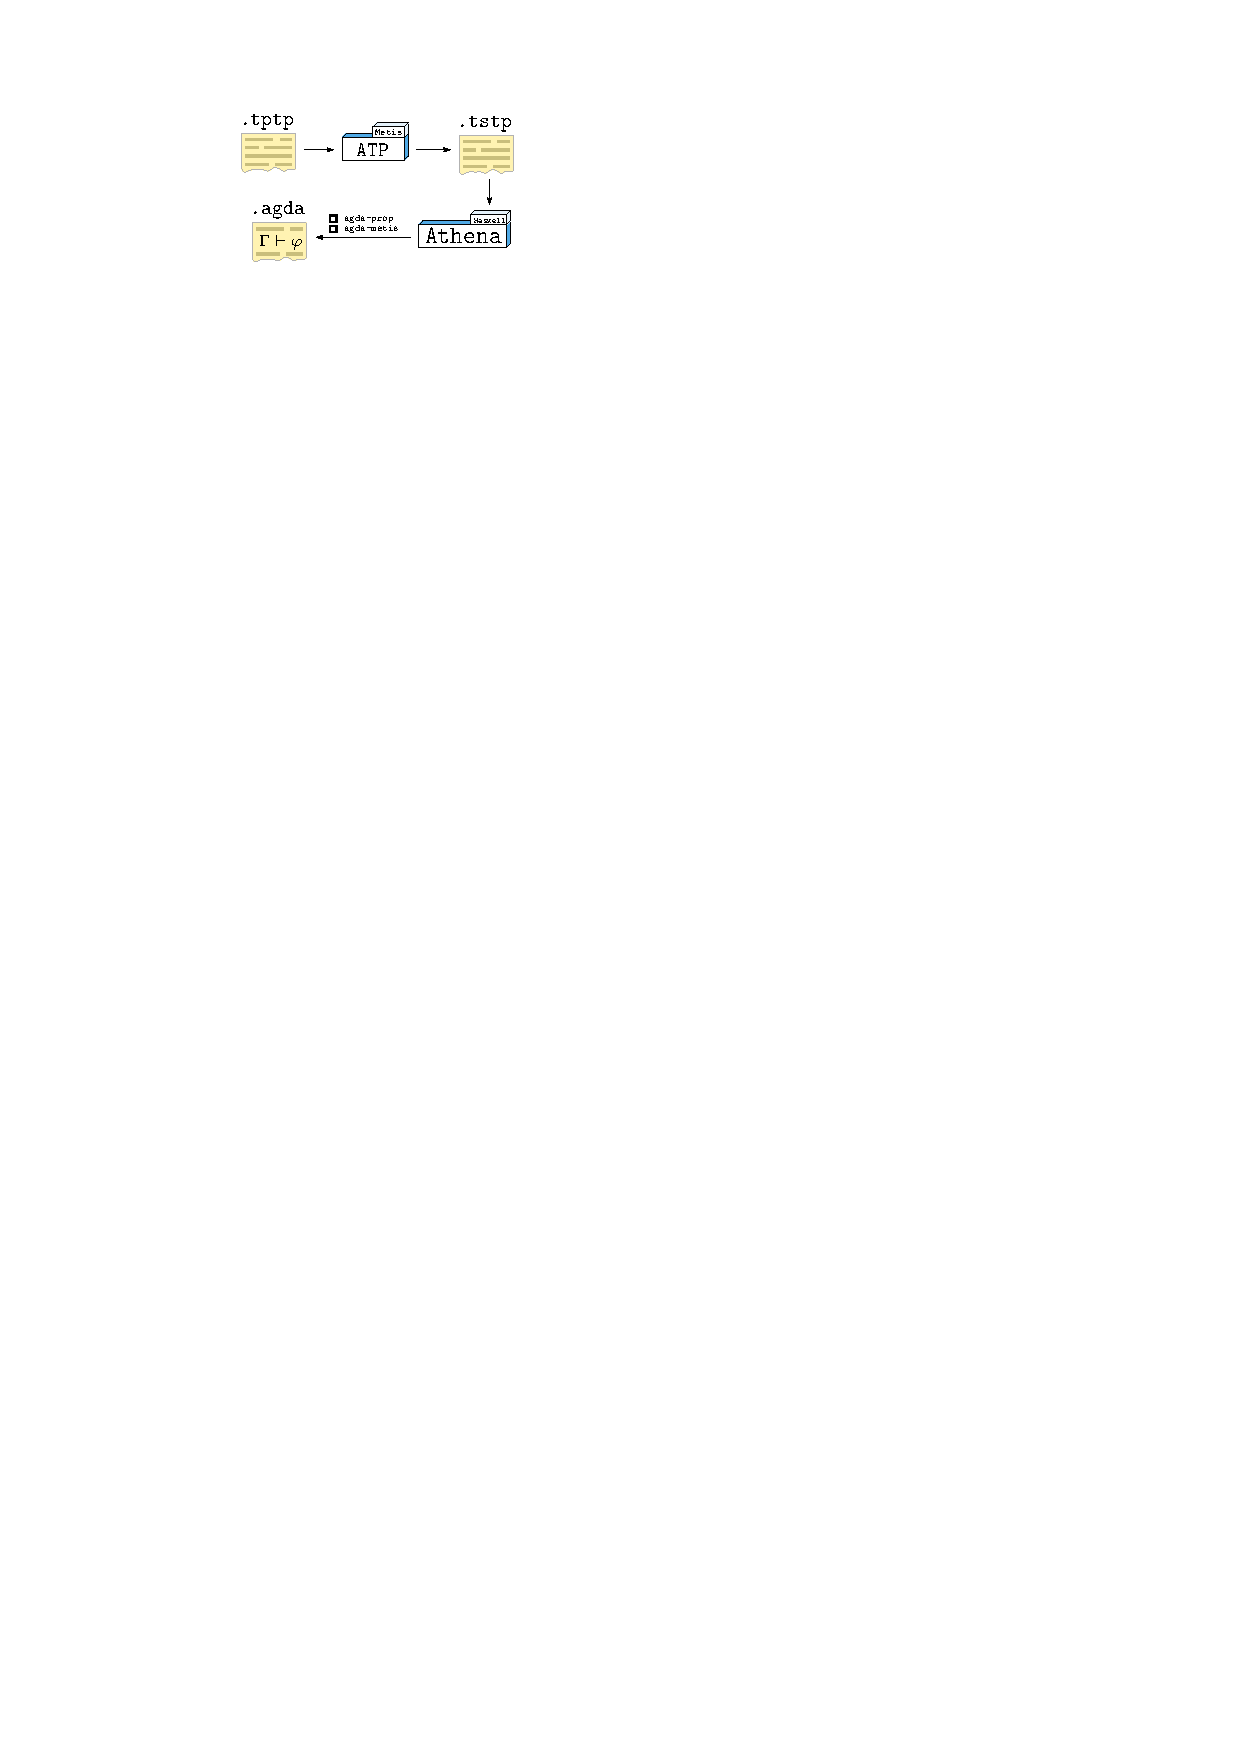
\includegraphics[scale=0.85]{diagram.pdf}
\label{im:athena}
\caption{Proof reconstruction work flow.}
\end{figure}
\end{frame}
% The tool : Athena.
% Its components:
% - agda-prop (logic framework)
% - agda-metis (ATP rules)
% - prop-pack (problems)

% Future work:
% - extend agda-prop to handle predicated logic
% - extend agda-metis to handle predicated proofs of Metis
% - reconstruct proofs of eprover: agda-eprover
% - support more versions of GHC in Athena.


\begin{frame}{References}

\end{frame}

\end{document}
